% Options for packages loaded elsewhere
\PassOptionsToPackage{unicode}{hyperref}
\PassOptionsToPackage{hyphens}{url}
\PassOptionsToPackage{dvipsnames,svgnames,x11names}{xcolor}
%
\documentclass[
]{article}

\usepackage{amsmath,amssymb}
\usepackage{iftex}
\ifPDFTeX
  \usepackage[T1]{fontenc}
  \usepackage[utf8]{inputenc}
  \usepackage{textcomp} % provide euro and other symbols
\else % if luatex or xetex
  \usepackage{unicode-math}
  \defaultfontfeatures{Scale=MatchLowercase}
  \defaultfontfeatures[\rmfamily]{Ligatures=TeX,Scale=1}
\fi
\usepackage{lmodern}
\ifPDFTeX\else  
    % xetex/luatex font selection
\fi
% Use upquote if available, for straight quotes in verbatim environments
\IfFileExists{upquote.sty}{\usepackage{upquote}}{}
\IfFileExists{microtype.sty}{% use microtype if available
  \usepackage[]{microtype}
  \UseMicrotypeSet[protrusion]{basicmath} % disable protrusion for tt fonts
}{}
\makeatletter
\@ifundefined{KOMAClassName}{% if non-KOMA class
  \IfFileExists{parskip.sty}{%
    \usepackage{parskip}
  }{% else
    \setlength{\parindent}{0pt}
    \setlength{\parskip}{6pt plus 2pt minus 1pt}}
}{% if KOMA class
  \KOMAoptions{parskip=half}}
\makeatother
\usepackage{xcolor}
\setlength{\emergencystretch}{3em} % prevent overfull lines
\setcounter{secnumdepth}{5}
% Make \paragraph and \subparagraph free-standing
\makeatletter
\ifx\paragraph\undefined\else
  \let\oldparagraph\paragraph
  \renewcommand{\paragraph}{
    \@ifstar
      \xxxParagraphStar
      \xxxParagraphNoStar
  }
  \newcommand{\xxxParagraphStar}[1]{\oldparagraph*{#1}\mbox{}}
  \newcommand{\xxxParagraphNoStar}[1]{\oldparagraph{#1}\mbox{}}
\fi
\ifx\subparagraph\undefined\else
  \let\oldsubparagraph\subparagraph
  \renewcommand{\subparagraph}{
    \@ifstar
      \xxxSubParagraphStar
      \xxxSubParagraphNoStar
  }
  \newcommand{\xxxSubParagraphStar}[1]{\oldsubparagraph*{#1}\mbox{}}
  \newcommand{\xxxSubParagraphNoStar}[1]{\oldsubparagraph{#1}\mbox{}}
\fi
\makeatother

\usepackage{color}
\usepackage{fancyvrb}
\newcommand{\VerbBar}{|}
\newcommand{\VERB}{\Verb[commandchars=\\\{\}]}
\DefineVerbatimEnvironment{Highlighting}{Verbatim}{commandchars=\\\{\}}
% Add ',fontsize=\small' for more characters per line
\usepackage{framed}
\definecolor{shadecolor}{RGB}{241,243,245}
\newenvironment{Shaded}{\begin{snugshade}}{\end{snugshade}}
\newcommand{\AlertTok}[1]{\textcolor[rgb]{0.68,0.00,0.00}{#1}}
\newcommand{\AnnotationTok}[1]{\textcolor[rgb]{0.37,0.37,0.37}{#1}}
\newcommand{\AttributeTok}[1]{\textcolor[rgb]{0.40,0.45,0.13}{#1}}
\newcommand{\BaseNTok}[1]{\textcolor[rgb]{0.68,0.00,0.00}{#1}}
\newcommand{\BuiltInTok}[1]{\textcolor[rgb]{0.00,0.23,0.31}{#1}}
\newcommand{\CharTok}[1]{\textcolor[rgb]{0.13,0.47,0.30}{#1}}
\newcommand{\CommentTok}[1]{\textcolor[rgb]{0.37,0.37,0.37}{#1}}
\newcommand{\CommentVarTok}[1]{\textcolor[rgb]{0.37,0.37,0.37}{\textit{#1}}}
\newcommand{\ConstantTok}[1]{\textcolor[rgb]{0.56,0.35,0.01}{#1}}
\newcommand{\ControlFlowTok}[1]{\textcolor[rgb]{0.00,0.23,0.31}{\textbf{#1}}}
\newcommand{\DataTypeTok}[1]{\textcolor[rgb]{0.68,0.00,0.00}{#1}}
\newcommand{\DecValTok}[1]{\textcolor[rgb]{0.68,0.00,0.00}{#1}}
\newcommand{\DocumentationTok}[1]{\textcolor[rgb]{0.37,0.37,0.37}{\textit{#1}}}
\newcommand{\ErrorTok}[1]{\textcolor[rgb]{0.68,0.00,0.00}{#1}}
\newcommand{\ExtensionTok}[1]{\textcolor[rgb]{0.00,0.23,0.31}{#1}}
\newcommand{\FloatTok}[1]{\textcolor[rgb]{0.68,0.00,0.00}{#1}}
\newcommand{\FunctionTok}[1]{\textcolor[rgb]{0.28,0.35,0.67}{#1}}
\newcommand{\ImportTok}[1]{\textcolor[rgb]{0.00,0.46,0.62}{#1}}
\newcommand{\InformationTok}[1]{\textcolor[rgb]{0.37,0.37,0.37}{#1}}
\newcommand{\KeywordTok}[1]{\textcolor[rgb]{0.00,0.23,0.31}{\textbf{#1}}}
\newcommand{\NormalTok}[1]{\textcolor[rgb]{0.00,0.23,0.31}{#1}}
\newcommand{\OperatorTok}[1]{\textcolor[rgb]{0.37,0.37,0.37}{#1}}
\newcommand{\OtherTok}[1]{\textcolor[rgb]{0.00,0.23,0.31}{#1}}
\newcommand{\PreprocessorTok}[1]{\textcolor[rgb]{0.68,0.00,0.00}{#1}}
\newcommand{\RegionMarkerTok}[1]{\textcolor[rgb]{0.00,0.23,0.31}{#1}}
\newcommand{\SpecialCharTok}[1]{\textcolor[rgb]{0.37,0.37,0.37}{#1}}
\newcommand{\SpecialStringTok}[1]{\textcolor[rgb]{0.13,0.47,0.30}{#1}}
\newcommand{\StringTok}[1]{\textcolor[rgb]{0.13,0.47,0.30}{#1}}
\newcommand{\VariableTok}[1]{\textcolor[rgb]{0.07,0.07,0.07}{#1}}
\newcommand{\VerbatimStringTok}[1]{\textcolor[rgb]{0.13,0.47,0.30}{#1}}
\newcommand{\WarningTok}[1]{\textcolor[rgb]{0.37,0.37,0.37}{\textit{#1}}}

\providecommand{\tightlist}{%
  \setlength{\itemsep}{0pt}\setlength{\parskip}{0pt}}\usepackage{longtable,booktabs,array}
\usepackage{calc} % for calculating minipage widths
% Correct order of tables after \paragraph or \subparagraph
\usepackage{etoolbox}
\makeatletter
\patchcmd\longtable{\par}{\if@noskipsec\mbox{}\fi\par}{}{}
\makeatother
% Allow footnotes in longtable head/foot
\IfFileExists{footnotehyper.sty}{\usepackage{footnotehyper}}{\usepackage{footnote}}
\makesavenoteenv{longtable}
\usepackage{graphicx}
\makeatletter
\def\maxwidth{\ifdim\Gin@nat@width>\linewidth\linewidth\else\Gin@nat@width\fi}
\def\maxheight{\ifdim\Gin@nat@height>\textheight\textheight\else\Gin@nat@height\fi}
\makeatother
% Scale images if necessary, so that they will not overflow the page
% margins by default, and it is still possible to overwrite the defaults
% using explicit options in \includegraphics[width, height, ...]{}
\setkeys{Gin}{width=\maxwidth,height=\maxheight,keepaspectratio}
% Set default figure placement to htbp
\makeatletter
\def\fps@figure{htbp}
\makeatother
% definitions for citeproc citations
\NewDocumentCommand\citeproctext{}{}
\NewDocumentCommand\citeproc{mm}{%
  \begingroup\def\citeproctext{#2}\cite{#1}\endgroup}
\makeatletter
 % allow citations to break across lines
 \let\@cite@ofmt\@firstofone
 % avoid brackets around text for \cite:
 \def\@biblabel#1{}
 \def\@cite#1#2{{#1\if@tempswa , #2\fi}}
\makeatother
\newlength{\cslhangindent}
\setlength{\cslhangindent}{1.5em}
\newlength{\csllabelwidth}
\setlength{\csllabelwidth}{3em}
\newenvironment{CSLReferences}[2] % #1 hanging-indent, #2 entry-spacing
 {\begin{list}{}{%
  \setlength{\itemindent}{0pt}
  \setlength{\leftmargin}{0pt}
  \setlength{\parsep}{0pt}
  % turn on hanging indent if param 1 is 1
  \ifodd #1
   \setlength{\leftmargin}{\cslhangindent}
   \setlength{\itemindent}{-1\cslhangindent}
  \fi
  % set entry spacing
  \setlength{\itemsep}{#2\baselineskip}}}
 {\end{list}}
\usepackage{calc}
\newcommand{\CSLBlock}[1]{\hfill\break\parbox[t]{\linewidth}{\strut\ignorespaces#1\strut}}
\newcommand{\CSLLeftMargin}[1]{\parbox[t]{\csllabelwidth}{\strut#1\strut}}
\newcommand{\CSLRightInline}[1]{\parbox[t]{\linewidth - \csllabelwidth}{\strut#1\strut}}
\newcommand{\CSLIndent}[1]{\hspace{\cslhangindent}#1}

\makeatletter
\@ifpackageloaded{caption}{}{\usepackage{caption}}
\AtBeginDocument{%
\ifdefined\contentsname
  \renewcommand*\contentsname{Table of contents}
\else
  \newcommand\contentsname{Table of contents}
\fi
\ifdefined\listfigurename
  \renewcommand*\listfigurename{List of Figures}
\else
  \newcommand\listfigurename{List of Figures}
\fi
\ifdefined\listtablename
  \renewcommand*\listtablename{List of Tables}
\else
  \newcommand\listtablename{List of Tables}
\fi
\ifdefined\figurename
  \renewcommand*\figurename{Figure}
\else
  \newcommand\figurename{Figure}
\fi
\ifdefined\tablename
  \renewcommand*\tablename{Table}
\else
  \newcommand\tablename{Table}
\fi
}
\@ifpackageloaded{float}{}{\usepackage{float}}
\floatstyle{ruled}
\@ifundefined{c@chapter}{\newfloat{codelisting}{h}{lop}}{\newfloat{codelisting}{h}{lop}[chapter]}
\floatname{codelisting}{Listing}
\newcommand*\listoflistings{\listof{codelisting}{List of Listings}}
\makeatother
\makeatletter
\makeatother
\makeatletter
\@ifpackageloaded{caption}{}{\usepackage{caption}}
\@ifpackageloaded{subcaption}{}{\usepackage{subcaption}}
\makeatother

\ifLuaTeX
  \usepackage{selnolig}  % disable illegal ligatures
\fi
\usepackage{bookmark}

\IfFileExists{xurl.sty}{\usepackage{xurl}}{} % add URL line breaks if available
\urlstyle{same} % disable monospaced font for URLs
\hypersetup{
  pdftitle={A Unified Framework for Multiple Component Cost-Effectiveness Models in R: A Tutorial},
  pdfauthor={Nathan Green},
  colorlinks=true,
  linkcolor={blue},
  filecolor={Maroon},
  citecolor={Blue},
  urlcolor={Blue},
  pdfcreator={LaTeX via pandoc}}


\title{A Unified Framework for Multiple Component Cost-Effectiveness
Models in R: A Tutorial}
\author{Nathan Green}
\date{}

\begin{document}
\maketitle
\begin{abstract}
\textbf{Background:} A cost-effectiveness analysis (CEA) compares an
intervention to one or more alternatives by estimating how much it costs
to gain an additional unit of health outcome. In recent years there has
been a shift in implementing these models in programmatic languages
better suited to more sophisticated models, model checking and advanced
visualisations.

\textbf{Problem:} It is common for a CEA model to consist of multiple
separate submodel components, such as those which combine decision trees
and Markov models. However, there are important limitations to the
traditional approach of implementing component models either disjointly
and manually passing input and output data between them, or as a single
ad-hoc script making clarity and testing a challenge.

\textbf{Solution:} We propose a unified framework that integrates these
submodels using declarative programming and S3 object-oriented
programming in the R programming language. This approach addresses
several issues associated with the separated or script-based approaches,
such as extensibility, flexibility, and efficiency. We provide a
detailed explanation of the unified framework and demonstrate its
practical application using a motivating example of a CEA model
involving multiple screening sessions over a lifetime where, at the
point of every screening session, individuals can be redistributed
across health states based on their screening results.

\textbf{Conclusions:} By better integrating component models, the
proposed framework enhances the robustness, transparency, and efficiency
of CEA, ultimately leading to improved informed decision-making in
healthcare and other fields.
\end{abstract}


\section{Introduction}\label{introduction}

Cost-effectiveness analysis (CEA) in healthcare is the comparative
assessment of alternative courses of action, evaluating both their
relative costs and downstream consequences (Drummond et al. 2015). To
conduct these evaluations, health economists frequently rely on
mathematical modelling. These models are becoming more powerful and
complex. One feature of this is that models may consist of multiple
linked components designed to capture different phases of a disease or
treatment pathway.

In particular, a widely used structural approach in CEA combines a
two-part model. This is particularly common when evaluating pathways
such as population screening programs or acute hospital care (Sandercock
et al. 2004). This consists of an initial stage where a decision-making
process and intervention are undertaken. An individual would be
evaluated and treated according to certain deterministic and random
considerations. The subsequent stage simulates the consequences of the
first stage on the population depending on the previous results (Briggs,
Claxton, and Sculpher 2006). For example, individuals may be invited to
screening and given treatment according to the results of an imperfect
test. Then their long term outcomes are estimated, with the population
split into true positive, true negative, false positive and false
negatives who may or may not have agreed to take the treatment which may
not have been effective. Outcomes for the second stage may include
progression to disease, side effects from treatment, and mortality.

There are general modelling and software engineering issues with the
legacy multiple component modelling approach. These are either disjoint
models or ad-hoc single scripts. This produces models which are error
prone, hard to test, reproduce or extend. In HTA projects it is often
required to modify or repurpose existing models, and the existing
approach can be inefficient and time consuming. In addition, it is usual
in a cost-effectiveness analysis to explore several (possibly many)
alternative interventions. Each of these may have different sets of unit
costs, health values, probabilities and possibly (but less common) model
structure. This would require the management of these alongside the
plugging in of model output as model inputs between components. The
analysis pipeline or workflow thus has potentially many `moving parts',
any one of which can introduce a bug or error which would affect the
calculation and the optimal decision.

There appears a consensus that modern code for health economics
modelling is not fit for purpose. Kent et al. (2019) and Wu et al.
(2019) argue that there is often a lack of clear code structure in
health economics models which makes it difficult for third parties to
validate them. We will propose an approach which solves this by making
the pipeline visible and not buried in nested loops. This sentiment is
repeated in Eddy et al. (2012), who state that a model should be
``reproducible by another team of investigators.'' Alarid-Escudero et
al. (2019) explicitly discuss the need for modularity, highlighting that
complex models should be broken down into reusable components to reduce
the risk of ``technical debt'' and error rates. Jalal et al. (2017)
discusses how although R is powerful it lacks a standard structure and
so modelling code is often poorer for it. They advocate for formal
structures to ensure models can be audited. Krijkamp et al. (2018)
provide a checklist that emphasizes modularity and input-output
consistency. We will propose a way to formalize the ``hand-off'' that is
usually handled with messy global variables.

Krijkamp et al. (2018) adopt a `bridge' or data translator function to
map between models. This formalises how to distribute individuals across
starting state of the long-term model. This is an improvement from the
hard-coded implementation often seen in other models. However, this is
still part of a sequential script rather than a formalised framework. We
propose going beyond simply `good coding style' to `software
engineering' practice. They manually chain components but this can be
managed or `orchestrated' automatically as part of the framework.

Although CEA models have been traditionally built in Microsoft Excel,
their increasing sophistication has driven a shift toward computational
programming languages like R (R Core Team 2025). Despite this
transition, the field has largely failed to adopt modern programming
paradigms. In particular, analysts often treat interconnected submodels
as isolated scripts, missing the opportunity to leverage the
architectural benefits of a programmatic framework. In software
engineering, integrating separate components into a unified system is a
well-established discipline that relies on a modular approach---breaking
a program into distinct, functional blocks which interact with one
another in standardised ways. Thus, a practical demonstration of how to
straightforwardly implement multi-component CEA models following
software engineering best practices could address this gap.

\section{General problem}\label{general-problem}

As an example which we will keep returning to in this article, we will
consider a particular type of the two-stage model already introduced.
This process can be represented with a decision tree model (DT) and
Markov model (MM). These are often used in combination to represent
acute or short-term, and chronic or long-term (population) impacts since
DTs do not explicitly represent time, unlike MM. An order of operation
is as follows:

\begin{enumerate}
\def\labelenumi{\roman{enumi}.}
\tightlist
\item
  Read in external data model inputs
\item
  Simulate the population sizes (or proportions) of the terminal state,
  and health and cost for the DT model
\item
  Pass the DT output to the MM as input
\item
  Simulate the health and cost values for the MM
\item
  Pass the DT and MM outputs to the Decision model
\item
  Process the combined results of the DT and MM
\item
  Repeat steps (i)-(vi) for a probabilistic sensitivity analysis (PSA)
\end{enumerate}

This process is represented in the flowchart in
Figure~\ref{fig-flowchart-combined}. The data may be passed amongst the
modules directly, which is reasonable with the same software.
Alternatively, the data may be stored externally in intermediate steps
and then read in when required. The diagram can be read roughly from
left to right, corresponding to (i) to (vi) above. It is not uncommon
for different submodels to be implemented in different software such as
MS Excel, R, Python, and Stata. We will not detail the inference stage
where the parameters of the model are estimated. This can be done in a
frequentist or Bayesian paradigm.

There are already several excellent tutorials on how to build simple DT
models or MM for cost-effectiveness analysis. The intention of this
paper is to build on these and develop the scope of applications to more
realistic problems encountered in industry and regulatory submissions.
It was sensible to start with simpler tutorials when people from other
software, such as MS Excel, are brought to programmatic implementations
such as R, but there is a desire now to further develop the available
toolkit and skill in the field.

\begin{figure}

\centering{

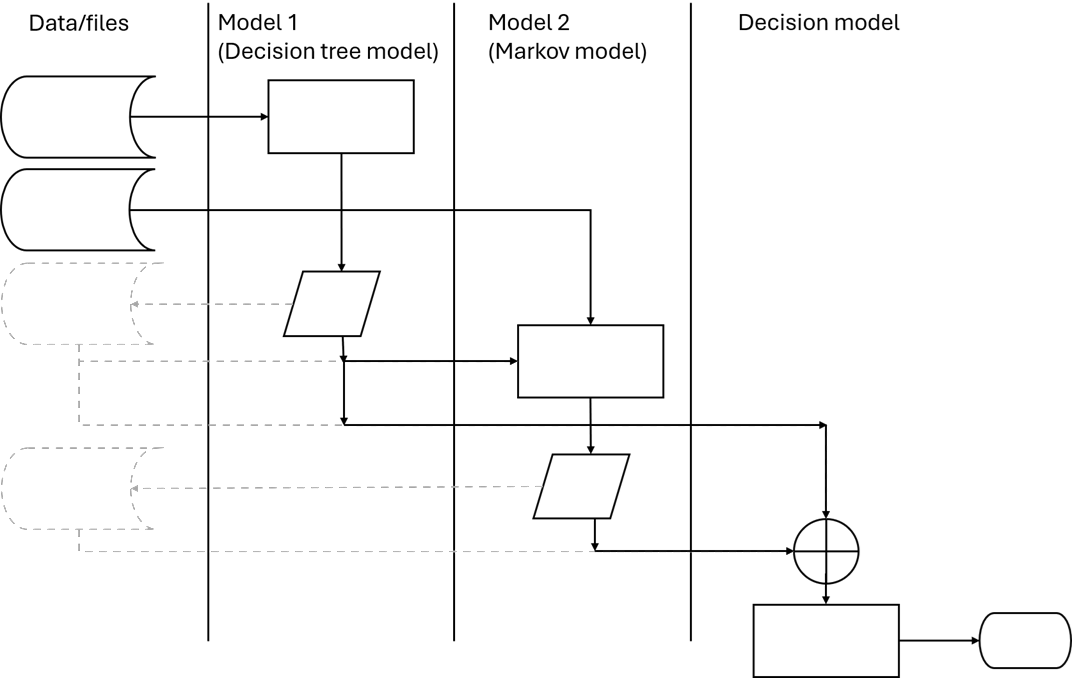
\includegraphics[width=0.9\textwidth,height=\textheight]{swimline-new.png}

}

\caption{\label{fig-flowchart-combined}Swimlane flowchart diagram for a
cost-effectiveness model comprised of a decision tree model followed by
a Markov model. Boxes represent processes; parallelograms are
input/output; cylinders are stored data; circle with cross is merge. The
solid lines indicate where the data are passed between modules directly,
and the grey dashed lines indicate where the data are passed between
modules via external file storage.}

\end{figure}%

\section{A unified framework}\label{a-unified-framework}

In this paper, we propose a unified and structured approach to building
cost-effectiveness models using declarative rather than imperative
programming. Unlike the traditional imperative approach --- where the
programmer manually manages every computational step to dictate how a
task is carried out --- declarative programming focuses on logically
describing what the program should accomplish. Key characteristics of
this approach include the abstraction of control flow and the automatic
handling of background implementation details. In the context of
unifying a decision tree (DT) and Markov model (MM), this framework
simplifies the simulation and cost-effectiveness calculations while
automatically managing the flow of data between modules.

This framework does not replace good modelling practice, such as
modularity, but rather supports and strengthens it. While some might
worry that bundling parts of a model together (i.e., increasing
``coupling'') can make code harder to manage, our framework is designed
to avoid these problems and instead promote clarity, reusability, and
scalability. Through reframing an existing model, we highlight the
benefits of moving to an object-oriented programming (OOP) approach.

In practical terms, this approach simplifies and clarifies key aspects
of the modelling process. Specifically, it streamlines how simulations
are executed (e.g., cohort transitions through a DT or MM), how costs
and health outcomes are calculated, and how data seamlessly flows
between distinct model components.

\section{S3 and object-oriented programming in
R}\label{s3-and-object-oriented-programming-in-r}

A cornerstone of our approach is the use of S3 OOP in R. The broader
statistical computing and data science communities have long leveraged
R's native S3 object-oriented system to unify disparate modelling
architectures, notably seen in the \emph{tidymodels} (Kuhn and Wickham
2020) ecosystem. Meanwhile, health technology assessment (HTA) tutorials
have largely overlooked this approach. Current HTA model development in
R typically relying on rigid, imperative scripting that mimics legacy
spreadsheet logic. We demonstrate how S3 method dispatch can serve as a
lightweight, native adaptor to seamlessly link sequential model
components (e.g., decision trees and Markov models) into a unified
pipeline. Table~\ref{tbl-s3classes} gives an overview of some common S3
object classes in R.

S3 OOP helps to manage model structure more cleanly. For instance, we
can define a \emph{generic} function like \texttt{print()} or
\texttt{summarize()} that works differently depending on the type of
object it is applied to (e.g., a DT vs.~a MM). R automatically chooses
the correct method based on the \emph{class} of the input, a process
known as method \emph{dispatch}. In R, S3 class is just a standard R
data structure (usually a list) that has a class attribute assigned to
it.

By decoupling the generic interface from its specific implementation,
this approach facilitates highly reusable code. Instead of maintaining
separate simulation functions for distinct model structures, an analyst
can define a single common interface. R's internal method dispatch
mechanism then automatically executes the correct subroutine. In OOP
terminology, this is called \emph{polymorphism}. This architectural
shift provides several key methodological advantages:

\begin{itemize}
\tightlist
\item
  \textbf{Unification:} Disparate model types (e.g., decision trees and
  Markov models) can be manipulated through a single, consistent syntax.
\item
  \textbf{Efficiency:} It minimizes code redundancy and reduces the risk
  of manual transcription errors.
\item
  \textbf{Maintainability:} It yields a modular codebase that is easier
  to debug, audit, and extend.
\item
  \textbf{Extensibility:} It permits the addition of novel model
  structures or summary functions without necessitating changes to the
  core logic.
\end{itemize}

Ultimately, deploying S3 object-oriented programming formalizes
cost-effectiveness models as distinct computational objects with
consistent behaviours, substantially enhancing analytical extensibility,
transparency and structural flexibility.

\begin{longtable}[]{@{}
  >{\raggedright\arraybackslash}p{(\columnwidth - 2\tabcolsep) * \real{0.5000}}
  >{\raggedright\arraybackslash}p{(\columnwidth - 2\tabcolsep) * \real{0.5000}}@{}}
\caption{Examples of S3 classes in R and how they are
defined.}\label{tbl-s3classes}\tabularnewline
\toprule\noalign{}
\begin{minipage}[b]{\linewidth}\raggedright
S3 Class
\end{minipage} & \begin{minipage}[b]{\linewidth}\raggedright
Description
\end{minipage} \\
\midrule\noalign{}
\endfirsthead
\toprule\noalign{}
\begin{minipage}[b]{\linewidth}\raggedright
S3 Class
\end{minipage} & \begin{minipage}[b]{\linewidth}\raggedright
Description
\end{minipage} \\
\midrule\noalign{}
\endhead
\bottomrule\noalign{}
\endlastfoot
\texttt{data.frame} & A tabular data structure with rows and columns.
Most common S3 class in R. \\
\texttt{lm} & Linear model object created by \texttt{lm()}. Stores
coefficients, residuals, etc. \\
\texttt{factor} & A categorical variable with levels. Internally stored
as integers with labels. \\
\texttt{ts} & Time-series object with time indexing. Used for modelling
temporal data. \\
\end{longtable}

\subsection{R code S3 example}\label{r-code-s3-example}

Below is a full example of using S3 method dispatch in R. We define a
custom generic function to print to the console \texttt{printModel()}
and two class-specific methods for objects of class
``\texttt{MarkovModel}'' and ``\texttt{DiseaseModel}''.

\begin{Shaded}
\begin{Highlighting}[]
\CommentTok{\# Create a generic function for printing model objects}
\NormalTok{printModel }\OtherTok{\textless{}{-}} \ControlFlowTok{function}\NormalTok{(x, ...) \{}
  \FunctionTok{UseMethod}\NormalTok{(}\StringTok{"printModel"}\NormalTok{)}
\NormalTok{\}}

\CommentTok{\# Method for class "MarkovModel"}
\NormalTok{printModel.MarkovModel }\OtherTok{\textless{}{-}} \ControlFlowTok{function}\NormalTok{(x, ...) \{}
  \FunctionTok{cat}\NormalTok{(}
    \StringTok{"A Markov model with states:"}\NormalTok{, }
    \FunctionTok{paste}\NormalTok{(x}\SpecialCharTok{$}\NormalTok{states, }\AttributeTok{collapse =} \StringTok{", "}\NormalTok{), }\StringTok{"}\SpecialCharTok{\textbackslash{}n}\StringTok{"}\NormalTok{)}
\NormalTok{\}}

\CommentTok{\# Method for class "DiseaseModel"}
\NormalTok{printModel.DiseaseModel }\OtherTok{\textless{}{-}} \ControlFlowTok{function}\NormalTok{(x, ...) \{}
  \FunctionTok{cat}\NormalTok{(}
    \StringTok{"Disease model states:"}\NormalTok{, }
    \FunctionTok{paste}\NormalTok{(x}\SpecialCharTok{$}\NormalTok{states, }\AttributeTok{collapse =} \StringTok{" {-}\textgreater{} "}\NormalTok{), }\StringTok{"}\SpecialCharTok{\textbackslash{}n}\StringTok{"}\NormalTok{)}
\NormalTok{\}}

\CommentTok{\# Define an object of class "MarkovModel"}
\NormalTok{x1 }\OtherTok{\textless{}{-}} \FunctionTok{list}\NormalTok{(}\AttributeTok{states =} \FunctionTok{c}\NormalTok{(}\StringTok{"Healthy"}\NormalTok{, }\StringTok{"Sick"}\NormalTok{, }\StringTok{"Dead"}\NormalTok{))}
\FunctionTok{class}\NormalTok{(x1) }\OtherTok{\textless{}{-}} \StringTok{"MarkovModel"}

\CommentTok{\# Define an object of class "DiseaseModel"}
\NormalTok{x2 }\OtherTok{\textless{}{-}} \FunctionTok{list}\NormalTok{(}\AttributeTok{states =} \FunctionTok{c}\NormalTok{(}\StringTok{"Mild"}\NormalTok{, }\StringTok{"Severe"}\NormalTok{, }\StringTok{"Death"}\NormalTok{))}
\FunctionTok{class}\NormalTok{(x2) }\OtherTok{\textless{}{-}} \StringTok{"DiseaseModel"}

\CommentTok{\# Call generic function {-}{-}{-}}

\CommentTok{\# Dispatches to printModel.MarkovModel}
\FunctionTok{printModel}\NormalTok{(x1)}
\end{Highlighting}
\end{Shaded}

\begin{verbatim}
A Markov model with states: Healthy, Sick, Dead 
\end{verbatim}

\begin{Shaded}
\begin{Highlighting}[]
\CommentTok{\# Dispatches to printModel.DiseaseModel}
\FunctionTok{printModel}\NormalTok{(x2)}
\end{Highlighting}
\end{Shaded}

\begin{verbatim}
Disease model states: Mild -> Severe -> Death 
\end{verbatim}

This demonstrates the core idea behind S3 where the method dispatch
depends on the class of the object passed to \texttt{printModel()}.
Additionally, objects can have more than one class and in this case
methods are dispatched in sequence.

Although the primary example in this paper focuses on using S3 to manage
macro-level workflows---specifically the integration of modular
\texttt{DecisionTree} and \texttt{MarkovModel} objects---the benefits of
OOP extend equally to micro-level data management. We strongly recommend
that analysts assign explicit classes to granular, user-defined types,
such as cost, QALY, or probability. In legacy imperative scripting,
health economists frequently rely on standard numeric arrays or data
frames, forcing them to clutter their functions with repetitive assert
or \texttt{stopifnot} statements to prevent silent data-type errors
(e.g., inadvertently multiplying a cost vector by another cost vector
instead of a probability). By replacing these fundamental inputs with S3
classes, analysts can leverage method dispatch to handle validation and
operations elegantly. For example, a generic \texttt{discount()} or
\texttt{convert\_country()} function can be designed to apply entirely
different logic depending on whether it receives a cost object or a QALY
object, ensuring robust, type-safe calculations throughout the model
pipeline.

\subsection{Model composition}\label{model-composition}

To use computer science terminology, \emph{function chaining} is a
common implementation of what is generally called function
\emph{composition} (mathematically written \(f(g(x))\)), especially in
object-oriented programming. In particular, a function that changes an
output to something that can be used as an input to the next function is
sometimes called a \emph{transformation} function. This is what is
required in our case to pipe from one model to the next. We can
elegantly chain models using S3 OOP.

\subsection{System architecture}\label{system-architecture}

In an OOP architecture, managing the data flow between distinct
components requires specific functional roles. To begin,
\emph{constructor} functions are required to instantiate the objects.
These functions take raw input data and format them into a classed
object (e.g., turning a standard list into a formal
\texttt{DecisionTree} or \texttt{MarkovModel} object) so that generic
functions know how to interact with it.

Once the objects are instantiated, linking different model components
seamlessly relies on the ``Adaptor pattern''. In software engineering,
an adaptor allows objects with incompatible interfaces to work together.
For health economists, this can be thought of as a standardized ``data
translator''.

For example, a DT might output a simple vector of patient proportions,
but a MM might require a specific starting cohort matrix. Rather than
cluttering the main analysis script with ad-hoc data manipulation code
to bridge this gap, the Adaptor pattern acts as a dedicated bridge. This
automatically converts the output of the source model into the exact
format expected by the target model. This is implemented by wrapping the
model execution in a function that handles the translation seamlessly
behind the scenes:

\begin{Shaded}
\begin{Highlighting}[]
\NormalTok{modelfun.modelclass }\OtherTok{\textless{}{-}} \ControlFlowTok{function}\NormalTok{(x, ...) \{}
\CommentTok{\# 1. Translate incoming data into a format the model needs}
\CommentTok{\# 2. Execute the model}
\CommentTok{\# 3. Translate results back into a standardized output format}
\NormalTok{\}}
\end{Highlighting}
\end{Shaded}

Finally, to manage the end-to-end execution of these linked models, an
\emph{orchestrator} function is employed. The orchestrator is
responsible for iterating through the chain of assembled models,
executing each one, and triggering the appropriate adaptors to pass the
output of one model directly into the input of the next.

\section{Case study: Multiple screening
episodes}\label{case-study-multiple-screening-episodes}

We reframe a previously published screening CEA model, built for the
purposes of teaching and training in R (Lin, O'Mahony, and Rosmalen
2023). The example will demonstrate the different implementation
approaches in a real-world case study. This is a CEA model that involves
multiple screening sessions over a lifetime where, at the point of every
screening session, individuals can be redistributed across health states
in a MM based on their screening results (Afonso et al. 2023; Hazen
2002; Hollenberg 1984).

\subsection{Data}\label{data}

The scenarios included are for five screening intervals of 2, 5, 10, 15,
20 years, and six total number of screening episodes 1, 2, 3, 4, 5, 10.
Figure~\ref{fig-screening-model} shows the high-level diagram of the
screening model from Lin, O'Mahony, and Rosmalen (2023). The Markov
model and decision tree diagrams are shown in
Figure~\ref{fig-markov-model} and Figure~\ref{fig-decision-tree-model}.

The data for the Markov model consist of the state transition
probability matrix \[
P = \begin{bmatrix}
0.9 & 0.05 & 0 & 0 & 0 & 0.05 \\
0 & 0.65 & 0.2 & 0 & 0.1 & 0.05 \\
0 & 0 & 0.6 & 0.20 & 0.2 & 0 \\
0 & 0 & 0 & 0.95 & 0 & 0.05 \\
0 & 0 & 0 & 0 & 1.0 & 0 \\
0 & 0 & 0 & 0 & 0 & 1
\end{bmatrix}
\] and the unit state cost and health attributes are \[
\mathbf{c}^{M} = (0, 0, 0, 100, 0, 0)^{\top}, \quad \mathbf{u}^{M} = (1, 0.8, 0.5, 0.9, 0, 0)^{\top}
\] The \(M\) superscript indicates that these are for the Markov model.
The data for the decision tree consist of the conditional transition
probabilities along each branch \[
\begin{aligned}
P(\text{FP} \mid \text{Healthy}) &= 0.1 \\
P(\text{TN} \mid \text{Healthy}) &= 0.9 \\[6pt]
P(\text{TP} \mid \text{Pre-clinical}) &= 0.7 \\
P(\text{FN} \mid \text{Pre-clinical}) &= 0.3 \\[6pt]
P(\text{TP} \mid \text{Disease}) &= 1.0 \\
P(\text{FN} \mid \text{Disease}) &= 0.0
\end{aligned}
\] and terminal state costs \(c^{D}(x) = 200\) if TP or FP, and
\(c^{D}(x) = 50\) if TN or FN. The \(D\) superscript indicates that
these are for the decision tree.

Finally, the initial distribution of individuals amongst the states of
the Markov model is defined as \[
\mathbf{\pi}_0 = (0.80, 0.15, 0.05, 0, 0, 0)^{\top}
\] Notice that the simulation begins with a decision tree model
screening round. The distribution of individuals at the start of a
screening episode is represented with the branches from the root node of
the decision tree which are therefore time-dependent.

\begin{figure}

\centering{

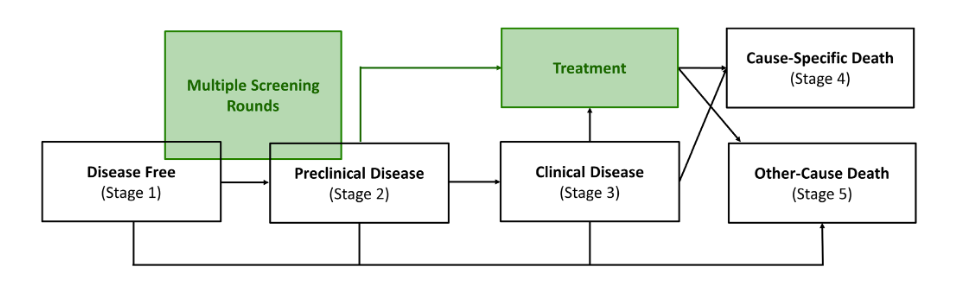
\includegraphics[width=1\textwidth,height=\textheight]{model-diagram.png}

}

\caption{\label{fig-screening-model}Screening model diagram taken from
Lin, O'Mahony, and Rosmalen (2023). The white health states represent
the natural history of disease. The two interventions, screening and
treatment, are labelled in green. The screening intervention can only be
implemented before the individual enters clinical health state (stage
3), and treatment can be received when patients are diagnosed from
screening (stage 2) or clinically presented (stage 3).}

\end{figure}%

\begin{figure}

\centering{

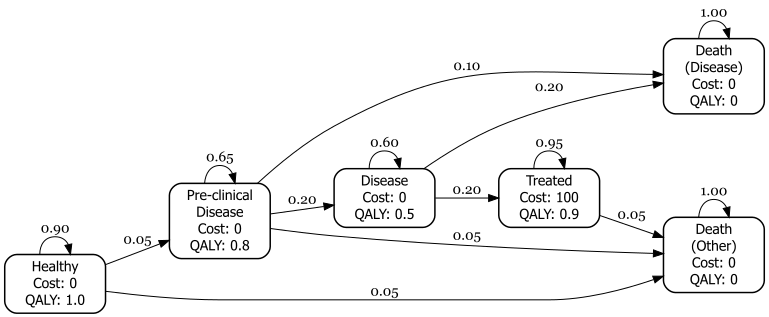
\includegraphics[width=1\textwidth,height=\textheight]{markov_model.png}

}

\caption{\label{fig-markov-model}Markov model component diagram for the
screening example.}

\end{figure}%

\begin{figure}

\centering{

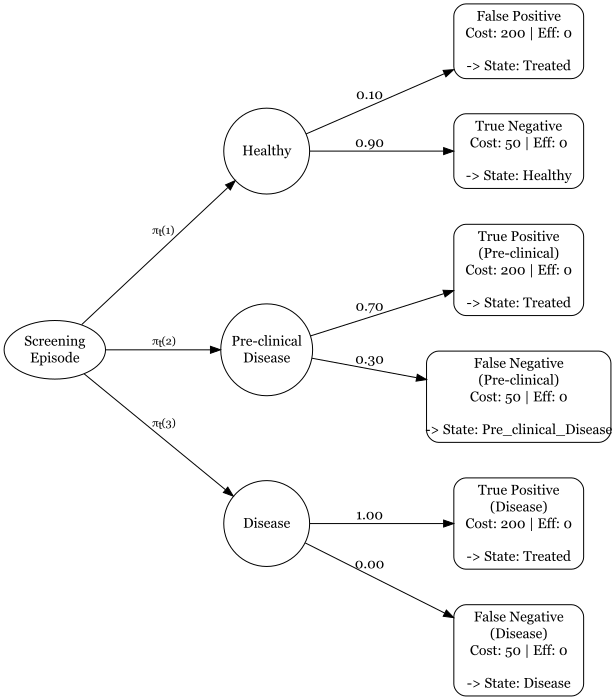
\includegraphics[width=1\textwidth,height=\textheight]{decision_tree_model2.png}

}

\caption{\label{fig-decision-tree-model}Decision tree model component
diagram for the screening example.}

\end{figure}%

\section{R implementation}\label{r-implementation}

The analysis was carried-out in R version 4.6.0. All code is available
on GitHub at \url{https://github.com/n8thangreen/modularce}. Because of
limited space and to focus the exposition, we do not include function
input checks (called \emph{asserts}) and other additional code, which it
is good practice to include.

The MM engine code is based on Green et al. (2023) and is considered a
black-box for our purposes. It is sufficient to define it in terms of
the \emph{contract}, that is, what values it requires as inputs and what
output we can expect to obtain from it. We will principally use base R
functions in the examples. This is to minimise the number of
dependencies and make the code more robust and reproducible. We consider
the CHEERS checklist (Husereau et al. 2022) for the key components of an
analysis which we need to take account of in our proposed framework. We
do not discount costs or health to present values for this simple model,
but in practice this is a core consideration.

\subsection{S3 Framework}\label{s3-framework}

The framework leverages the S3 methodology to seamlessly transition
patient cohorts. At each screening interval (2, 5, 10, 15, and 20
years), the DT calculates the immediate redistribution of individuals
based on test outcomes. Instead of manual data hand-offs, the
\texttt{update\_model()} generic function captures these revised
proportions and feeds them directly into the MM. This allows the MM to
project long-term downstream costs and health outcomes continuously
without breaking the computational pipeline.

The class constructor functions for a decision tree and a Markov model
are:

\begin{Shaded}
\begin{Highlighting}[]
\NormalTok{DecisionTree }\OtherTok{\textless{}{-}} \ControlFlowTok{function}\NormalTok{(data, }\AttributeTok{disc\_rate =} \FloatTok{0.035}\NormalTok{) \{}
  \FunctionTok{structure}\NormalTok{(}
    \FunctionTok{list}\NormalTok{(}\AttributeTok{data =}\NormalTok{ data,}
         \AttributeTok{discount\_rate =}\NormalTok{ disc\_rate),}
    \AttributeTok{class =} \FunctionTok{c}\NormalTok{(}\StringTok{"DecisionTree"}\NormalTok{, }\StringTok{"Model"}\NormalTok{))}
\NormalTok{\}}

\NormalTok{MarkovModel }\OtherTok{\textless{}{-}} \ControlFlowTok{function}\NormalTok{(trans\_matrix, }
\NormalTok{                        costs, utils, }
                        \AttributeTok{init\_probs =} \ConstantTok{NULL}\NormalTok{, }
                        \AttributeTok{mapping =} \ConstantTok{NULL}\NormalTok{, }
                        \AttributeTok{n\_cycles =} \DecValTok{2}\NormalTok{, }
                        \AttributeTok{disc\_rate =} \FloatTok{0.035}\NormalTok{) \{}
  \FunctionTok{structure}\NormalTok{(}
    \FunctionTok{list}\NormalTok{(}
      \AttributeTok{trans\_matrix  =}\NormalTok{ trans\_matrix,}
      \AttributeTok{cost\_vector   =}\NormalTok{ costs,}
      \AttributeTok{util\_vector   =}\NormalTok{ utils,}
      \AttributeTok{init\_probs    =}\NormalTok{ init\_probs,}
      \AttributeTok{mapping       =}\NormalTok{ mapping,}
      \AttributeTok{n\_cycles      =}\NormalTok{ n\_cycles,}
      \AttributeTok{discount\_rate =}\NormalTok{ disc\_rate}
\NormalTok{    ),}
    \AttributeTok{class =} \FunctionTok{c}\NormalTok{(}\StringTok{"MarkovModel"}\NormalTok{, }\StringTok{"Model"}\NormalTok{)}
\NormalTok{  )}
\NormalTok{\}}
\end{Highlighting}
\end{Shaded}

The \texttt{structure()} function defines an object with additional
attributes, in this case class.

We will also create a \texttt{CombinedModel()} constructor which will
simply consist of a list of other models which have previously been
created with their own class constructors as above. This structure will
allow us to pass around a single object.

\begin{Shaded}
\begin{Highlighting}[]
\NormalTok{CombinedModel }\OtherTok{\textless{}{-}} \ControlFlowTok{function}\NormalTok{(...) \{}
  \FunctionTok{structure}\NormalTok{(}\FunctionTok{list}\NormalTok{(...), }
            \AttributeTok{class =} \FunctionTok{c}\NormalTok{(}\StringTok{"CombinedModel"}\NormalTok{, }\StringTok{"Model"}\NormalTok{))}
\NormalTok{\}}
\end{Highlighting}
\end{Shaded}

We next define the generic functions, which are the polymorphic methods
which will behave differently depending on what class of object is
passed to them. This is `boilerplate' R code which takes the same format
every time.

\begin{Shaded}
\begin{Highlighting}[]
\NormalTok{run\_model }\OtherTok{\textless{}{-}} \ControlFlowTok{function}\NormalTok{(model, ...) \{}
  \FunctionTok{UseMethod}\NormalTok{(}\StringTok{"run\_model"}\NormalTok{)}
\NormalTok{\}}

\NormalTok{update\_model }\OtherTok{\textless{}{-}} \ControlFlowTok{function}\NormalTok{(model, result) \{}
  \FunctionTok{UseMethod}\NormalTok{(}\StringTok{"update\_model"}\NormalTok{)}
\NormalTok{\}}
\end{Highlighting}
\end{Shaded}

The class-specific \texttt{run\_model()} methods for each of the
submodels are defined next:

\begin{Shaded}
\begin{Highlighting}[]
\NormalTok{run\_model.MarkovModel }\OtherTok{\textless{}{-}} \ControlFlowTok{function}\NormalTok{(model, ...) \{}
\NormalTok{  out }\OtherTok{\textless{}{-}} \FunctionTok{markov\_model}\NormalTok{(}
    \AttributeTok{start\_pop     =}\NormalTok{ model}\SpecialCharTok{$}\NormalTok{init\_probs,}
    \AttributeTok{trans\_mat     =}\NormalTok{ model}\SpecialCharTok{$}\NormalTok{trans\_matrix,}
    \AttributeTok{cost\_vec      =}\NormalTok{ model}\SpecialCharTok{$}\NormalTok{cost\_vector,}
    \AttributeTok{util\_vec      =}\NormalTok{ model}\SpecialCharTok{$}\NormalTok{util\_vector,}
    \AttributeTok{n\_cycles      =}\NormalTok{ model}\SpecialCharTok{$}\NormalTok{n\_cycles,}
    \AttributeTok{discount\_rate =}\NormalTok{ model}\SpecialCharTok{$}\NormalTok{discount\_rate,}
    \AttributeTok{start\_cycle   =} \FunctionTok{ifelse}\NormalTok{(}\FunctionTok{is.null}\NormalTok{(model}\SpecialCharTok{$}\NormalTok{start\_cycle), }\DecValTok{0}\NormalTok{, model}\SpecialCharTok{$}\NormalTok{start\_cycle)}
\NormalTok{  )}
  
  \FunctionTok{list}\NormalTok{(}
    \AttributeTok{expected\_cost =}\NormalTok{ out}\SpecialCharTok{$}\NormalTok{expected\_cost,}
    \AttributeTok{expected\_eff  =}\NormalTok{ out}\SpecialCharTok{$}\NormalTok{expected\_eff,}
    \AttributeTok{terminal      =}\NormalTok{ out}\SpecialCharTok{$}\NormalTok{final\_state,}
    \AttributeTok{trace         =}\NormalTok{ out}\SpecialCharTok{$}\NormalTok{trace,}
    \AttributeTok{time\_elapsed  =}\NormalTok{ model}\SpecialCharTok{$}\NormalTok{n\_cycles}
\NormalTok{  )}
\NormalTok{\}}

\NormalTok{run\_model.DecisionTree }\OtherTok{\textless{}{-}} \ControlFlowTok{function}\NormalTok{(model, ...) \{}
\NormalTok{  pathways }\OtherTok{\textless{}{-}} \FunctionTok{calculate\_pathways}\NormalTok{(model}\SpecialCharTok{$}\NormalTok{data)}
  
\NormalTok{  start\_cycle }\OtherTok{\textless{}{-}} \FunctionTok{ifelse}\NormalTok{(}\FunctionTok{is.null}\NormalTok{(model}\SpecialCharTok{$}\NormalTok{start\_cycle), }\DecValTok{0}\NormalTok{, model}\SpecialCharTok{$}\NormalTok{start\_cycle)}
\NormalTok{  discount\_factor }\OtherTok{\textless{}{-}} \DecValTok{1} \SpecialCharTok{/}\NormalTok{ (}\DecValTok{1} \SpecialCharTok{+}\NormalTok{ model}\SpecialCharTok{$}\NormalTok{discount\_rate)}\SpecialCharTok{\^{}}\NormalTok{start\_cycle}
  
  \FunctionTok{list}\NormalTok{(}
    \AttributeTok{expected\_cost =} \FunctionTok{sum}\NormalTok{(pathways}\SpecialCharTok{$}\NormalTok{prob }\SpecialCharTok{*}\NormalTok{ pathways}\SpecialCharTok{$}\NormalTok{cost) }\SpecialCharTok{*}\NormalTok{ discount\_factor,}
    \AttributeTok{expected\_eff  =} \FunctionTok{sum}\NormalTok{(pathways}\SpecialCharTok{$}\NormalTok{prob }\SpecialCharTok{*}\NormalTok{ pathways}\SpecialCharTok{$}\NormalTok{eff) }\SpecialCharTok{*}\NormalTok{ discount\_factor,}
    \AttributeTok{path\_results  =}\NormalTok{ pathways,}
    \AttributeTok{time\_elapsed  =} \DecValTok{0}
\NormalTok{  )}
\NormalTok{\}}
\end{Highlighting}
\end{Shaded}

As already stated, we assume the internal simulation engines of the
decision tree, \texttt{calculate\_pathways()}, and Markov model,
\texttt{markov\_model()}, as black boxes for our purposes. The full code
is all available in the GitHub repo.

Next, we define the adaptor functions for each of the submodels. These
are model-specific functions derived from the generic
\texttt{update\_model()}. In each case, results from the previous model
in the pipeline are passed in and adapted appropriately to be input for
the subsequent model, as defined by the class of the first argument.

\begin{Shaded}
\begin{Highlighting}[]
\NormalTok{update\_model.MarkovModel }\OtherTok{\textless{}{-}} \ControlFlowTok{function}\NormalTok{(model, prev\_result) \{}
  \ControlFlowTok{if}\NormalTok{ (}\SpecialCharTok{!}\FunctionTok{is.null}\NormalTok{(prev\_result}\SpecialCharTok{$}\NormalTok{path\_results) }\SpecialCharTok{\&\&} \SpecialCharTok{!}\FunctionTok{is.null}\NormalTok{(model}\SpecialCharTok{$}\NormalTok{mapping)) \{}
\NormalTok{    all\_nm }\OtherTok{\textless{}{-}} \FunctionTok{colnames}\NormalTok{(model}\SpecialCharTok{$}\NormalTok{trans\_matrix)}
\NormalTok{    new\_init }\OtherTok{\textless{}{-}} \FunctionTok{setNames}\NormalTok{(}\FunctionTok{rep}\NormalTok{(}\DecValTok{0}\NormalTok{, }\FunctionTok{length}\NormalTok{(all\_nm)), all\_nm)}
    
\NormalTok{    paths }\OtherTok{\textless{}{-}}\NormalTok{ prev\_result}\SpecialCharTok{$}\NormalTok{path\_results}
\NormalTok{    paths}\SpecialCharTok{$}\NormalTok{state }\OtherTok{\textless{}{-}}\NormalTok{ model}\SpecialCharTok{$}\NormalTok{mapping[paths}\SpecialCharTok{$}\NormalTok{terminal\_node]}
    
    \CommentTok{\# Sum the probabilities for each state}
    \ControlFlowTok{for}\NormalTok{ (s }\ControlFlowTok{in} \FunctionTok{unique}\NormalTok{(paths}\SpecialCharTok{$}\NormalTok{state)) \{}
\NormalTok{      new\_init[s] }\OtherTok{\textless{}{-}} \FunctionTok{sum}\NormalTok{(paths}\SpecialCharTok{$}\NormalTok{prob[paths}\SpecialCharTok{$}\NormalTok{state }\SpecialCharTok{==}\NormalTok{ s])}
\NormalTok{    \}}
    
\NormalTok{    model}\SpecialCharTok{$}\NormalTok{init\_probs }\OtherTok{\textless{}{-}}\NormalTok{ new\_init}
\NormalTok{  \}}
\NormalTok{  model}
\NormalTok{\}}

\NormalTok{update\_model.DecisionTree }\OtherTok{\textless{}{-}} \ControlFlowTok{function}\NormalTok{(model, prev\_result) \{}
  \ControlFlowTok{if}\NormalTok{ (}\SpecialCharTok{!}\FunctionTok{is.null}\NormalTok{(prev\_result}\SpecialCharTok{$}\NormalTok{terminal)) \{}
\NormalTok{    end\_states }\OtherTok{\textless{}{-}}\NormalTok{ prev\_result}\SpecialCharTok{$}\NormalTok{terminal}
\NormalTok{    tree }\OtherTok{\textless{}{-}}\NormalTok{ model}\SpecialCharTok{$}\NormalTok{data}
\NormalTok{    root\_idx }\OtherTok{\textless{}{-}} \FunctionTok{which}\NormalTok{(}
\NormalTok{      tree}\SpecialCharTok{$}\NormalTok{from }\SpecialCharTok{==} \StringTok{"root"} \SpecialCharTok{\&} 
\NormalTok{        tree}\SpecialCharTok{$}\NormalTok{to }\SpecialCharTok{\%in\%} \FunctionTok{names}\NormalTok{(end\_states))}
\NormalTok{    tree}\SpecialCharTok{$}\NormalTok{prob[root\_idx] }\OtherTok{\textless{}{-}}\NormalTok{ end\_states[tree}\SpecialCharTok{$}\NormalTok{to[root\_idx]]}
\NormalTok{    model}\SpecialCharTok{$}\NormalTok{data }\OtherTok{\textless{}{-}}\NormalTok{ tree}
\NormalTok{  \}}
\NormalTok{  model}
\NormalTok{\}}
\end{Highlighting}
\end{Shaded}

The final key element is the orchestrator function. This higher-level
function takes as first argument an object of class
\texttt{CombinedModel} and steps through each of the component submodels
by running and updating data for the appropriate submodel-specific
methods of \texttt{run\_model()} and \texttt{update\_model()}.

\begin{Shaded}
\begin{Highlighting}[]
\NormalTok{run\_model.CombinedModel }\OtherTok{\textless{}{-}} \ControlFlowTok{function}\NormalTok{(model, ...) \{}
\NormalTok{  results }\OtherTok{\textless{}{-}} \FunctionTok{list}\NormalTok{()}
\NormalTok{  current\_time }\OtherTok{\textless{}{-}} \DecValTok{0}  \CommentTok{\# initialise internal clock}
  
  \ControlFlowTok{for}\NormalTok{ (i }\ControlFlowTok{in} \FunctionTok{seq\_along}\NormalTok{(model)) \{}
\NormalTok{    curr\_model }\OtherTok{\textless{}{-}}\NormalTok{ model[[i]]}
    
    \CommentTok{\# stamps model with current time}
\NormalTok{    curr\_model}\SpecialCharTok{$}\NormalTok{start\_cycle }\OtherTok{\textless{}{-}}\NormalTok{ current\_time}
    
    \ControlFlowTok{if}\NormalTok{ (i }\SpecialCharTok{\textgreater{}} \DecValTok{1}\NormalTok{) \{}
\NormalTok{      curr\_model }\OtherTok{\textless{}{-}} \FunctionTok{update\_model}\NormalTok{(curr\_model, results[[i }\SpecialCharTok{{-}} \DecValTok{1}\NormalTok{]])}
\NormalTok{    \}}

\NormalTok{    res }\OtherTok{\textless{}{-}} \FunctionTok{run\_model}\NormalTok{(curr\_model)}
\NormalTok{    results[[i]] }\OtherTok{\textless{}{-}}\NormalTok{ res}
    
    \CommentTok{\# advance clock using self{-}reported elapsed time}
\NormalTok{    current\_time }\OtherTok{\textless{}{-}}\NormalTok{ current\_time }\SpecialCharTok{+}\NormalTok{ res}\SpecialCharTok{$}\NormalTok{time\_elapsed}
\NormalTok{  \}}
\NormalTok{  results}
\NormalTok{\}}
\end{Highlighting}
\end{Shaded}

\subsection{Input data}\label{input-data}

Now that the function preparatory code is complete, the input data as
defined in the Data section above are translated into R code. We define
a simulation duration of 20 years and define the screening programme in
terms of the time between screening and the number of screening
episodes. The analysis will investigate all combinations of intervals
and episode values.

\begin{Shaded}
\begin{Highlighting}[]
\CommentTok{\# Define the grid of parameters}
\NormalTok{time\_horizon }\OtherTok{\textless{}{-}} \DecValTok{20}
\NormalTok{t\_between\_screens }\OtherTok{\textless{}{-}} \DecValTok{1}\SpecialCharTok{:}\DecValTok{10}
\NormalTok{num\_screens }\OtherTok{\textless{}{-}} \DecValTok{1}\SpecialCharTok{:}\DecValTok{10}
\CommentTok{\# t\_between\_screens \textless{}{-} c(2, 5, 10, 15, 20)}
\CommentTok{\# num\_screens \textless{}{-} c(1, 2, 3, 4, 5, 10)}
\CommentTok{\# Set your new discount rate}
\NormalTok{discount\_rate }\OtherTok{\textless{}{-}} \FloatTok{0.035}
\end{Highlighting}
\end{Shaded}

The decision tree data are defined as a \texttt{tribble()} from the
\emph{tibble} package which allows us to write it in the same format
that it will be printed for clearer code (\textbf{?@fig-code-input-dt}).

\begin{Shaded}
\begin{Highlighting}[]
\NormalTok{decision\_tree }\OtherTok{\textless{}{-}}\NormalTok{ tibble}\SpecialCharTok{::}\FunctionTok{tribble}\NormalTok{(}
  \SpecialCharTok{\textasciitilde{}}\NormalTok{from,                  }\SpecialCharTok{\textasciitilde{}}\NormalTok{to,                    }\SpecialCharTok{\textasciitilde{}}\NormalTok{prob, }\SpecialCharTok{\textasciitilde{}}\NormalTok{cost, }\SpecialCharTok{\textasciitilde{}}\NormalTok{eff,}
  \StringTok{"root"}\NormalTok{,                 }\StringTok{"Healthy"}\NormalTok{,              }\FloatTok{0.80}\NormalTok{,      }\DecValTok{0}\NormalTok{,    }\DecValTok{0}\NormalTok{,}
  \StringTok{"root"}\NormalTok{,                 }\StringTok{"Pre\_clinical\_Disease"}\NormalTok{, }\FloatTok{0.15}\NormalTok{,      }\DecValTok{0}\NormalTok{,    }\DecValTok{0}\NormalTok{,  }\CommentTok{\# Markov model}
  \StringTok{"root"}\NormalTok{,                 }\StringTok{"Disease"}\NormalTok{,              }\FloatTok{0.05}\NormalTok{,      }\DecValTok{0}\NormalTok{,    }\DecValTok{0}\NormalTok{,  }\CommentTok{\# state }
  \StringTok{"root"}\NormalTok{,                 }\StringTok{"Treated"}\NormalTok{,              }\FloatTok{0.00}\NormalTok{,      }\DecValTok{0}\NormalTok{,    }\DecValTok{0}\NormalTok{,  }\CommentTok{\# distribution}
  \StringTok{"root"}\NormalTok{,                 }\StringTok{"Death\_from\_Disease"}\NormalTok{,   }\FloatTok{0.00}\NormalTok{,      }\DecValTok{0}\NormalTok{,    }\DecValTok{0}\NormalTok{,  }
  \StringTok{"root"}\NormalTok{,                 }\StringTok{"Other\_Cause\_Death"}\NormalTok{,    }\FloatTok{0.00}\NormalTok{,      }\DecValTok{0}\NormalTok{,    }\DecValTok{0}\NormalTok{,}
  \StringTok{"Healthy"}\NormalTok{,              }\StringTok{"FP"}\NormalTok{,                   }\FloatTok{0.10}\NormalTok{,    }\DecValTok{200}\NormalTok{,    }\DecValTok{0}\NormalTok{,  }\CommentTok{\# False Positive}
  \StringTok{"Healthy"}\NormalTok{,              }\StringTok{"TN"}\NormalTok{,                   }\FloatTok{0.90}\NormalTok{,     }\DecValTok{50}\NormalTok{,    }\DecValTok{0}\NormalTok{,  }\CommentTok{\# True Negative}
  \StringTok{"Pre\_clinical\_Disease"}\NormalTok{, }\StringTok{"TP\_Preclinical"}\NormalTok{,       }\FloatTok{0.70}\NormalTok{,    }\DecValTok{200}\NormalTok{,    }\DecValTok{0}\NormalTok{,  }\CommentTok{\# True Positive}
  \StringTok{"Pre\_clinical\_Disease"}\NormalTok{, }\StringTok{"FN\_Preclinical"}\NormalTok{,       }\FloatTok{0.30}\NormalTok{,     }\DecValTok{50}\NormalTok{,    }\DecValTok{0}\NormalTok{,  }\CommentTok{\# False Negative}
  \StringTok{"Disease"}\NormalTok{,              }\StringTok{"TP\_Disease"}\NormalTok{,           }\FloatTok{1.00}\NormalTok{,    }\DecValTok{200}\NormalTok{,    }\DecValTok{0}\NormalTok{,  }\CommentTok{\# True Positive}
  \StringTok{"Disease"}\NormalTok{,              }\StringTok{"FN\_Disease"}\NormalTok{,           }\FloatTok{0.00}\NormalTok{,     }\DecValTok{50}\NormalTok{,    }\DecValTok{0}   \CommentTok{\# False Negative}
\NormalTok{)}
\end{Highlighting}
\end{Shaded}

The Markov model transition probability matrix is defined in
\textbf{?@fig-code-input-mm}.

\begin{Shaded}
\begin{Highlighting}[]
\NormalTok{states }\OtherTok{\textless{}{-}} \FunctionTok{c}\NormalTok{(}
  \StringTok{"Healthy"}\NormalTok{, }\StringTok{"Pre\_clinical\_Disease"}\NormalTok{, }\StringTok{"Disease"}\NormalTok{, }\StringTok{"Treated"}\NormalTok{, }\StringTok{"Death\_from\_Disease"}\NormalTok{, }
  \StringTok{"Other\_Cause\_Death"}\NormalTok{)}

\NormalTok{trans\_mat }\OtherTok{\textless{}{-}} \FunctionTok{matrix}\NormalTok{(}
  \FunctionTok{c}\NormalTok{(}
    \CommentTok{\#    H     P     D     T     DD    OCD}
    \FloatTok{0.90}\NormalTok{, }\FloatTok{0.05}\NormalTok{, }\FloatTok{0.00}\NormalTok{, }\FloatTok{0.00}\NormalTok{, }\FloatTok{0.00}\NormalTok{, }\FloatTok{0.05}\NormalTok{, }\CommentTok{\# Healthy (H)}
    \FloatTok{0.00}\NormalTok{, }\FloatTok{0.65}\NormalTok{, }\FloatTok{0.20}\NormalTok{, }\FloatTok{0.00}\NormalTok{, }\FloatTok{0.10}\NormalTok{, }\FloatTok{0.05}\NormalTok{, }\CommentTok{\# Pre{-}clinical Disease (P)}
    \FloatTok{0.00}\NormalTok{, }\FloatTok{0.00}\NormalTok{, }\FloatTok{0.60}\NormalTok{, }\FloatTok{0.20}\NormalTok{, }\FloatTok{0.20}\NormalTok{, }\FloatTok{0.00}\NormalTok{, }\CommentTok{\# Clinical Disease (D)}
    \FloatTok{0.00}\NormalTok{, }\FloatTok{0.00}\NormalTok{, }\FloatTok{0.00}\NormalTok{, }\FloatTok{0.95}\NormalTok{, }\FloatTok{0.00}\NormalTok{, }\FloatTok{0.05}\NormalTok{, }\CommentTok{\# Treated (T)}
    \FloatTok{0.00}\NormalTok{, }\FloatTok{0.00}\NormalTok{, }\FloatTok{0.00}\NormalTok{, }\FloatTok{0.00}\NormalTok{, }\FloatTok{1.00}\NormalTok{, }\FloatTok{0.00}\NormalTok{, }\CommentTok{\# Death from Disease (DD) {-} Absorbing}
    \FloatTok{0.00}\NormalTok{, }\FloatTok{0.00}\NormalTok{, }\FloatTok{0.00}\NormalTok{, }\FloatTok{0.00}\NormalTok{, }\FloatTok{0.00}\NormalTok{, }\FloatTok{1.00}  \CommentTok{\# Other{-}Cause Death (OCD) {-} Absorbing}
\NormalTok{  ),}
  \AttributeTok{nrow =} \DecValTok{6}\NormalTok{, }\AttributeTok{byrow =} \ConstantTok{TRUE}\NormalTok{,}
  \AttributeTok{dimnames =} \FunctionTok{list}\NormalTok{(}\AttributeTok{from =}\NormalTok{ states, }
                  \AttributeTok{to =}\NormalTok{ states)}
\NormalTok{)}
\end{Highlighting}
\end{Shaded}

The state cost and health values are defined as follows:

\begin{Shaded}
\begin{Highlighting}[]
\NormalTok{cost\_vec }\OtherTok{\textless{}{-}} \FunctionTok{c}\NormalTok{(}
  \AttributeTok{Healthy              =} \DecValTok{0}\NormalTok{,}
  \AttributeTok{Pre\_clinical\_Disease =} \DecValTok{0}\NormalTok{,}
  \AttributeTok{Disease              =} \DecValTok{0}\NormalTok{,}
  \AttributeTok{Treated              =} \DecValTok{100}\NormalTok{,}
  \AttributeTok{Death\_from\_Disease   =} \DecValTok{0}\NormalTok{,}
  \AttributeTok{Other\_Cause\_Death    =} \DecValTok{0}
\NormalTok{)}

\NormalTok{util\_vec }\OtherTok{\textless{}{-}} \FunctionTok{c}\NormalTok{(}
  \AttributeTok{Healthy              =} \FloatTok{1.0}\NormalTok{,}
  \AttributeTok{Pre\_clinical\_Disease =} \FloatTok{0.8}\NormalTok{,}
  \AttributeTok{Disease              =} \FloatTok{0.5}\NormalTok{,}
  \AttributeTok{Treated              =} \FloatTok{0.9}\NormalTok{,}
  \AttributeTok{Death\_from\_Disease   =} \FloatTok{0.0}\NormalTok{,}
  \AttributeTok{Other\_Cause\_Death    =} \FloatTok{0.0}
\NormalTok{)}

\CommentTok{\# Cohort distribution for natural history}
\NormalTok{init\_pop }\OtherTok{\textless{}{-}} \FunctionTok{c}\NormalTok{(}
  \AttributeTok{Healthy              =} \FloatTok{1.0}\NormalTok{,}
  \AttributeTok{Pre\_clinical\_Disease =} \FloatTok{0.0}\NormalTok{,}
  \AttributeTok{Disease              =} \FloatTok{0.0}\NormalTok{,}
  \AttributeTok{Treated              =} \FloatTok{0.0}\NormalTok{,}
  \AttributeTok{Death\_from\_Disease   =} \FloatTok{0.0}\NormalTok{,}
  \AttributeTok{Other\_Cause\_Death    =} \FloatTok{0.0}
\NormalTok{)}
\end{Highlighting}
\end{Shaded}

Finally, we need to define the mapping from the decision tree terminal
nodes to the Markov model states:

\begin{Shaded}
\begin{Highlighting}[]
\NormalTok{mapping }\OtherTok{\textless{}{-}} \FunctionTok{c}\NormalTok{(}
  \AttributeTok{FP                 =} \StringTok{"Treated"}\NormalTok{,}
  \AttributeTok{TN                 =} \StringTok{"Healthy"}\NormalTok{,}
  \AttributeTok{TP\_Preclinical     =} \StringTok{"Treated"}\NormalTok{,}
  \AttributeTok{FN\_Preclinical     =} \StringTok{"Pre\_clinical\_Disease"}\NormalTok{,}
  \AttributeTok{TP\_Disease         =} \StringTok{"Treated"}\NormalTok{,}
  \AttributeTok{FN\_Disease         =} \StringTok{"Disease"}\NormalTok{,}
  \AttributeTok{Death\_from\_Disease =} \StringTok{"Death\_from\_Disease"}\NormalTok{,}
  \AttributeTok{Other\_Cause\_Death  =} \StringTok{"Other\_Cause\_Death"}\NormalTok{,}
  \AttributeTok{Treated            =} \StringTok{"Treated"}
\NormalTok{)}
\end{Highlighting}
\end{Shaded}

\subsection{Analysis}\label{analysis}

Having established the simulation code and input data, it is
straightforward to run the analysis inside of a loop over the scenarios.

\begin{Shaded}
\begin{Highlighting}[]
\CommentTok{\# Loop through scenarios and execute the unified framework}

\NormalTok{all\_results }\OtherTok{\textless{}{-}} \FunctionTok{list}\NormalTok{()}
\NormalTok{dt }\OtherTok{\textless{}{-}} \FunctionTok{DecisionTree}\NormalTok{(decision\_tree, }\AttributeTok{disc\_rate =}\NormalTok{ discount\_rate)}

\ControlFlowTok{for}\NormalTok{ (t\_val }\ControlFlowTok{in}\NormalTok{ t\_between\_screens) \{}
\NormalTok{  mm\_scenario }\OtherTok{\textless{}{-}} 
    \FunctionTok{MarkovModel}\NormalTok{(}\AttributeTok{trans\_matrix =}\NormalTok{ trans\_mat,}
                \AttributeTok{costs =}\NormalTok{ cost\_vec,}
                \AttributeTok{utils =}\NormalTok{ util\_vec,}
                \AttributeTok{init\_probs =}\NormalTok{ init\_pop,}
                \AttributeTok{mapping =}\NormalTok{ mapping,}
                \AttributeTok{n\_cycles =}\NormalTok{ t\_val,}
                \AttributeTok{disc\_rate =}\NormalTok{ discount\_rate)}
  
  \ControlFlowTok{for}\NormalTok{ (n\_scr }\ControlFlowTok{in}\NormalTok{ num\_screens) \{}
\NormalTok{    total\_screen\_time }\OtherTok{\textless{}{-}}\NormalTok{ n\_scr }\SpecialCharTok{*}\NormalTok{ t\_val}
    
    \CommentTok{\# Filter out impossible combinations that}
    \CommentTok{\# exceed the 20{-}year time horizon}
    \ControlFlowTok{if}\NormalTok{ (total\_screen\_time }\SpecialCharTok{\textgreater{}}\NormalTok{ time\_horizon) }\ControlFlowTok{next}
    
\NormalTok{    submodels }\OtherTok{\textless{}{-}} \FunctionTok{rep}\NormalTok{(}\FunctionTok{list}\NormalTok{(dt, mm\_scenario), n\_scr)}
    
\NormalTok{    t\_remain }\OtherTok{\textless{}{-}}\NormalTok{ time\_horizon }\SpecialCharTok{{-}}\NormalTok{ total\_screen\_time}
    \ControlFlowTok{if}\NormalTok{ (t\_remain }\SpecialCharTok{\textgreater{}} \DecValTok{0}\NormalTok{) \{}
\NormalTok{      submodels[[}\FunctionTok{length}\NormalTok{(submodels)]]}\SpecialCharTok{$}\NormalTok{n\_cycles }\OtherTok{\textless{}{-}}\NormalTok{ t\_val }\SpecialCharTok{+}\NormalTok{ t\_remain}
\NormalTok{    \}}
    
\NormalTok{    screening\_model }\OtherTok{\textless{}{-}} \FunctionTok{do.call}\NormalTok{(CombinedModel, }\AttributeTok{args =}\NormalTok{ submodels)}
    
\NormalTok{    results\_scenario }\OtherTok{\textless{}{-}} \FunctionTok{run\_model}\NormalTok{(screening\_model)}
    
\NormalTok{    result\_label }\OtherTok{\textless{}{-}} \FunctionTok{paste0}\NormalTok{(}\StringTok{"t\_between\_"}\NormalTok{, t\_val, }\StringTok{"\_screens\_"}\NormalTok{, n\_scr)}
    
\NormalTok{    all\_results[[result\_label]] }\OtherTok{\textless{}{-}} \FunctionTok{list}\NormalTok{(}
      \AttributeTok{t\_between\_screens =}\NormalTok{ t\_val,}
      \AttributeTok{num\_screens       =}\NormalTok{ n\_scr,}
      \AttributeTok{results           =}\NormalTok{ results\_scenario}
\NormalTok{    )}
\NormalTok{  \}}
\NormalTok{\}}
\end{Highlighting}
\end{Shaded}

\subsection{Probabilistic sensitivity
analysis}\label{probabilistic-sensitivity-analysis}

Probabilistic Sensitivity Analysis (PSA) is fundamentally streamlined
under our unified framework. In a traditional basic approach, analysts
must manually manage the extraction of DT outputs to feed into the MM
for every single PSA iteration, which is both error-prone and
computationally inefficient. By encapsulating the model within the
\texttt{CombinedModel} class, a PSA simply requires applying a mapping
function (such as \texttt{lapply()} in base R) over the probabilistic
input distributions. The \texttt{run\_model.CombinedModel()} function
acts as the orchestrator, automatically handling the internal control
flow and data passing for each iteration. This ensures that structural
integrity is maintained across thousands of simulation runs without
manual intervention.

\subsection{Design choices}\label{design-choices}

Even within the proposed architecture there are several subjective
design decisions to make, which can depend on the specifics of the
problem at hand. One design choice is where in the code to perform the
linking of models. One option is to chain the models together when we
create them or another option is to do this at the same time as running
the model. There are pros and cons to each approach.

Another issue is to do with the generalisability of linking models.
Should the code use the information about which type of model is being
linked from (source) and linked to (target)? In an OOP framework this
would require something called \emph{double dispatch} which is not the
original intention of S3 in R but can be manufactured using it and is
implemented in packages such as \emph{vctrs} (Wickham, Henry, and
Vaughan 2026). Taking into account these considerations, in our case
study example we have placed the linking logic within the model running
function. We have also assumed that given a target model, we then know
what the source model is. This is reasonable in our context and keeps
the code clean for demonstration purposes. An alternative version of our
code using the double dispatch approach employed by \emph{vctrs} is also
available in the supplementary material. The newer and less adopted S7
OOP system in R does natively support multiple dispatch which could
elegantly solve the problem with a little more advanced code. We provide
a version of the code in the supplementary material.

Our decision to utilize an S3-based orchestrator to link sequential
model components aligns with established best practices in modern R
software engineering. For instance, the \emph{tidymodels} ecosystem
(specifically the \emph{workflows} and \emph{stacks} packages) relies
heavily on S3 generics to handle the sequential passing of data between
preprocessing steps, individual models, and ensemble meta-models.

A Unified Markup Language (UML) diagram of the code structure is given
in Appendix Figure~\ref{fig-UML}. This shows how all of the functions
are related to each other.

\section{Results}\label{results}

Figure~\ref{fig-occupy-combined} illustrates the state occupancy over a
20-year time horizon for the 2-year and 10-year screening intervals.
These plots demonstrate the expected dynamics: more frequent screening
redistributes the population more rapidly into the ``Treated'' and
``Disease'' states.

\begin{figure}

\begin{minipage}{\linewidth}

\centering{

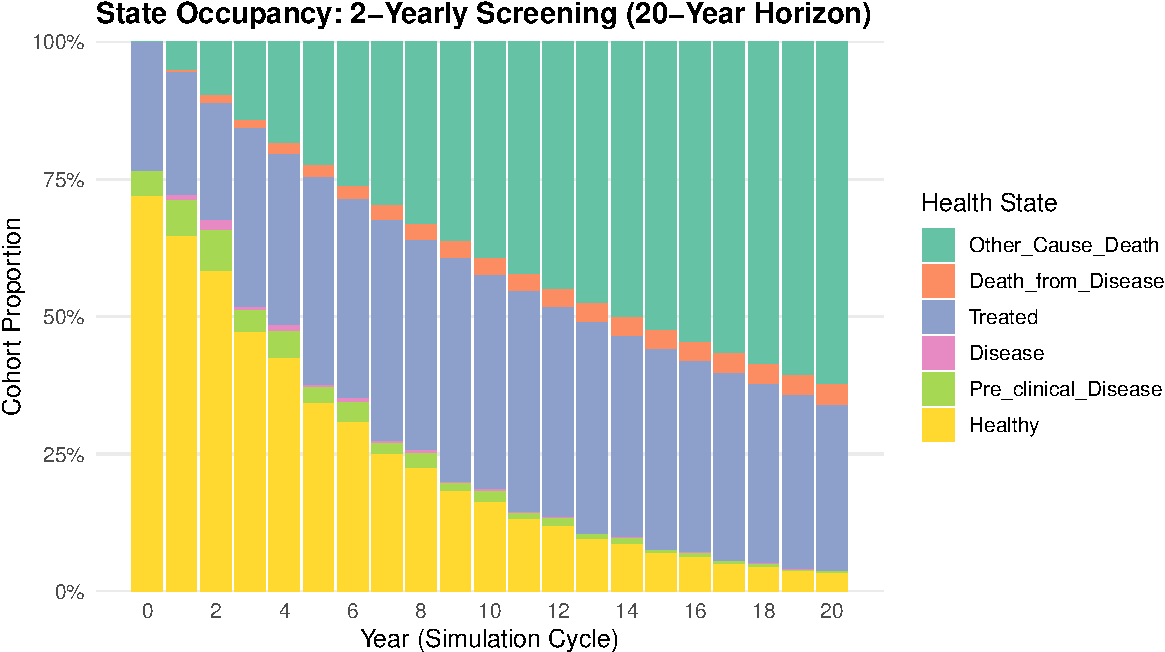
\includegraphics{manuscript_files/figure-pdf/fig-occupy-combined-1.pdf}

}

\subcaption{\label{fig-occupy-combined-1}2-yearly screening (10 rounds,
20-year horizon)}

\end{minipage}%
\newline
\begin{minipage}{\linewidth}

\centering{

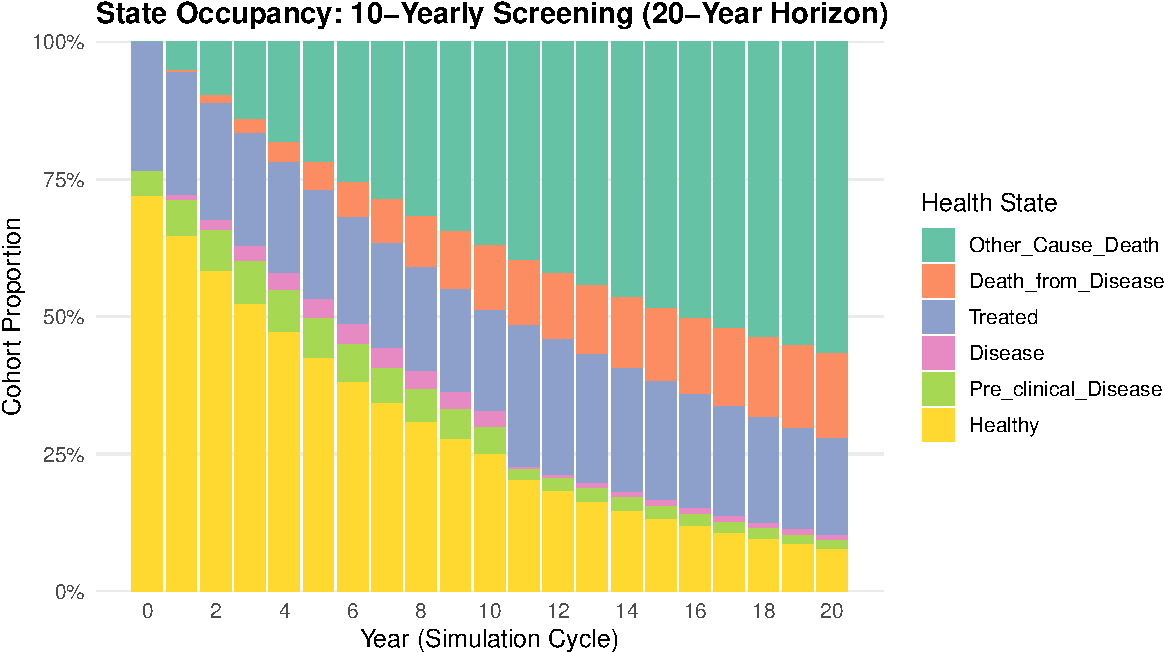
\includegraphics{manuscript_files/figure-pdf/fig-occupy-combined-2.pdf}

}

\subcaption{\label{fig-occupy-combined-2}10-yearly screening (2 rounds,
20-year horizon)}

\end{minipage}%

\caption{\label{fig-occupy-combined}State occupancy plots comparing
2-year and 10-year screening intervals.}

\end{figure}%

Figure~\ref{fig-ce-plot} synthesizes the cost-effectiveness across the
full grid of evaluated screening strategies, plotting total accumulated
costs against total health outcomes. As expected from a structurally
sound health economic evaluation, the results display clear efficiency
trade-offs. Strategies utilizing highly frequent screening intervals
(e.g., the 2-year interval curve) yield the highest overall health
benefits by capturing clinical transitions earlier, but they do so at a
significantly steeper marginal cost trajectory due to compounding
screening and treatment expenses. Conversely, less frequent screening
(e.g., the 15- and 20-year intervals) produces lower-cost outcomes with
correspondingly reduced health gains.

Importantly, the smooth and mathematically predictable progression of
these curves---scaling logically with the number of screening
episodes---demonstrates that the declarative S3 framework functions
exactly as intended. It confirms that the object-oriented architecture
correctly accumulates costs and propagates complex cohort transitions
between the DT and MM without the silent data-loss or misallocation
errors common in manual imperative scripts.

\begin{figure}

\centering{

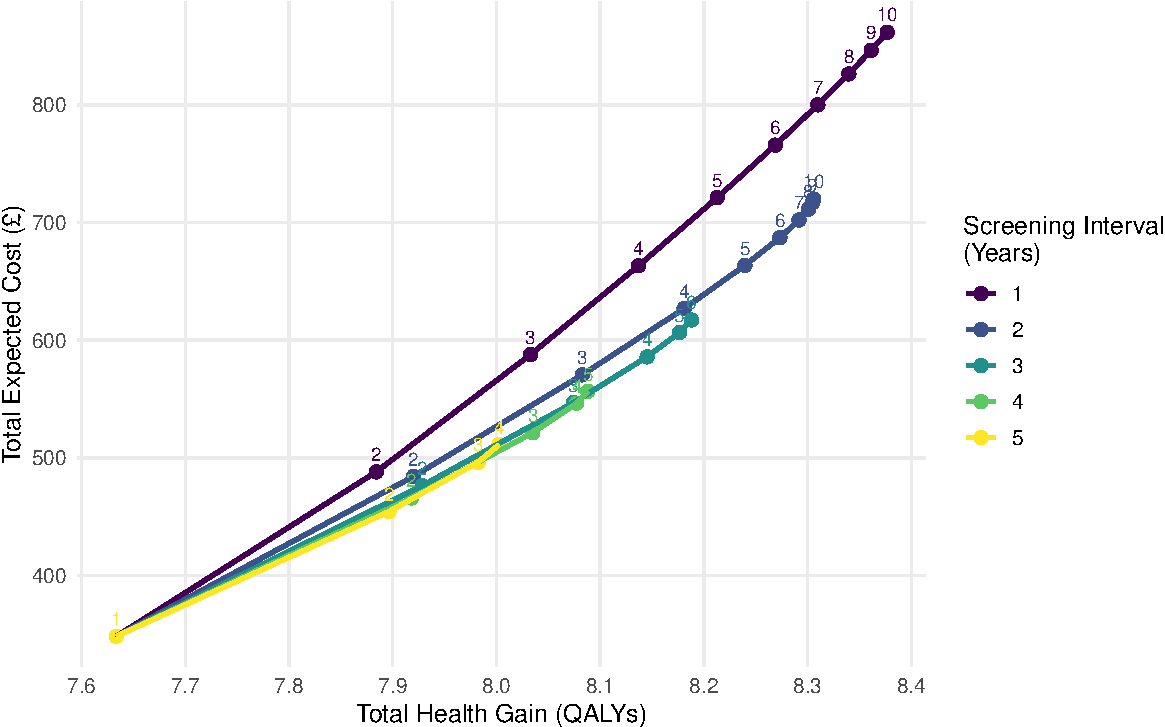
\includegraphics{manuscript_files/figure-pdf/fig-ce-plot-1.pdf}

}

\caption{\label{fig-ce-plot}Cost-effectiveness plot for screening
intervals of 1 to 5 years, with all screening episodes numbered.}

\end{figure}%

\section{Conclusion}\label{conclusion}

We have demonstrated that adopting a declarative, object-oriented
programming approach using S3 in R provides a robust and scalable
solution for multi-component cost-effectiveness models. By abstracting
the control flow and automating data transitions between DTs and MMs,
this framework directly addresses the testability, reproducibility, and
efficiency issues prevalent in legacy imperative scripts. Although
moving away from traditional step-by-step coding requires a paradigm
shift for many health economists, the resulting unified architecture
aligns health technology assessment with modern software engineering
best practices. Ultimately, this improves the transparency, flexibility,
and reliability of the models used to inform critical healthcare
decisions.

\subsection*{Acknowledgements}\label{acknowledgements}
\addcontentsline{toc}{subsection}{Acknowledgements}

xxx

\subsection*{References}\label{references}
\addcontentsline{toc}{subsection}{References}

\phantomsection\label{refs}
\begin{CSLReferences}{1}{0}
\bibitem[\citeproctext]{ref-Afonso2023}
Afonso, D, H Davies, B Avey, and S Mealing. 2023. {``{MSR8 Nesting a
Decision Tree into a Markov Model Structure: An Alternative Way of
Tracking Movement in a Diagnostic Model}.''} \emph{Value Heal.} 26 (12):
S394. \url{https://doi.org/10.1016/j.jval.2023.09.2067}.

\bibitem[\citeproctext]{ref-AlaridEscudero2019}
Alarid-Escudero, Fernando, Eline M. Krijkamp, Eva A. Enns, Alan Yang, M.
G. Myriam Hunink, Petros Pechlivanoglou, and Hawre J. Jalal. 2019. {``A
Framework for Decision-Analytic Modeling in {R}: Implementing Tertiary
Prevention of Colorectal Cancer with a {Markov} Model.''} \emph{Medical
Decision Making} 39 (2): 175--84.
\url{https://doi.org/10.1177/0272989X18814775}.

\bibitem[\citeproctext]{ref-briggs2006decision}
Briggs, Andrew, Karl Claxton, and Mark Sculpher. 2006. \emph{Decision
Modelling for Health Economic Evaluation}. Oxford, UK: Oxford University
Press.

\bibitem[\citeproctext]{ref-drummond2015methods}
Drummond, Michael F., Mark J. Sculpher, Karl Claxton, Greg L. Stoddart,
and George W. Torrance. 2015. \emph{Methods for the Economic Evaluation
of Health Care Programmes}. 4th ed. Oxford, UK: Oxford University Press.

\bibitem[\citeproctext]{ref-Eddy2012MDM}
Eddy, David M., William Hollingworth, J. Jaime Caro, Robert Itzler, and
Mark S. Townsend. 2012. {``Model Transparency and Validation: A Report
of the {ISPOR-SMDM} Modeling Good Research Practices Task Force--7.''}
\emph{Medical Decision Making} 32 (5): 733--43.
\url{https://doi.org/10.1177/0272989X12454504}.

\bibitem[\citeproctext]{ref-Green2023}
Green, Nathan, Felicity Lamrock, Niamh Naylor, Miqdad Asaria, Mark
Strong, Chris Taylor, Dougie van der Wielen, and Marta O. Soares. 2023.
{``Health Economic Evaluation Using Markov Models in r for Microsoft
Excel Users: A Tutorial.''} \emph{PharmacoEconomics} 41 (1): 5--19.
\url{https://doi.org/10.1007/s40273-022-01199-7}.

\bibitem[\citeproctext]{ref-Hazen2002}
Hazen, Gordon B. 2002. {``{Stochastic Trees and the StoTree Modeling
Environment: Models and Software for Medical Decision Analysis}.''}
\emph{J. Med. Syst.} 26 (5).

\bibitem[\citeproctext]{ref-hollenberg1984markov}
Hollenberg, JP. 1984. {``Markov Cycle Trees-a New Representation for
Complex Markov-Processes.''} In \emph{Medical Decision Making},
4:529--29. 4. Hanley \& Belfus Inc 210 S 13th St, Philadelphia, PA
19107.

\bibitem[\citeproctext]{ref-husereau_consolidated_2022}
Husereau, Don, Michael Drummond, Federico Augustovski, Esther de
Bekker-Grob, Andrew H. Briggs, Chris Carswell, Lisa Caulley, et al.
2022. {``Consolidated {Health} {Economic} {Evaluation} {Reporting}
{Standards} 2022 ({CHEERS} 2022) {Statement}: {Updated} {Reporting}
{Guidance} for {Health} {Economic} {Evaluations}.''} \emph{Value in
Health} 25 (January): 3--9.
\url{https://doi.org/10.1016/j.jval.2021.11.1349}.

\bibitem[\citeproctext]{ref-Jalal2017}
Jalal, Hawre, Petros Pechlivanoglou, Eline Krijkamp, Fernando
Alarid-Escudero, Eva Enns, and M. G. Myriam Hunink. 2017. {``An Overview
of {R} in Health Decision Sciences.''} \emph{Medical Decision Making} 37
(7): 735--46. \url{https://doi.org/10.1177/0272989X16679605}.

\bibitem[\citeproctext]{ref-Kent2019}
Kent, Seamus, Frauke Becker, Talitha Feenstra, An Tran-Duy, Iryna
Schlackow, Michelle Tew, Ping Zhang, et al. 2019. {``The Challenge of
Transparency and Validation in Health Economic Decision Modelling: A
View from Mount Hood.''} \emph{PharmacoEconomics} 37 (11): 1305--12.
\url{https://doi.org/10.1007/s40273-019-00825-1}.

\bibitem[\citeproctext]{ref-Krijkamp2018}
Krijkamp, Eline M., Fernando Alarid-Escudero, Eva A. Enns, Hawre J.
Jalal, M. G. Myriam Hunink, and Petros Pechlivanoglou. 2018. {``A
Checklist for Generating, Reporting and Modelling Decision-Analytic
Models in {R}.''} \emph{Medical Decision Making} 38 (8): 1000--1012.
\url{https://doi.org/10.1177/0272989X18811838}.

\bibitem[\citeproctext]{ref-tidymodels}
Kuhn, Max, and Hadley Wickham. 2020. \emph{Tidymodels: A Collection of
Packages for Modeling and Machine Learning Using Tidyverse Principles.}
\url{https://www.tidymodels.org}.

\bibitem[\citeproctext]{ref-lin2023simple}
Lin, Y. S., J. F. O'Mahony, and J. van Rosmalen. 2023. {``A Simple
Cost-Effectiveness Model of Screening: An Open-Source Teaching and
Research Tool Coded in {R}.''} \emph{PharmacoEconomics - Open} 7 (4):
507--23. \url{https://doi.org/10.1007/s41669-023-00414-1}.

\bibitem[\citeproctext]{ref-rlanguage}
R Core Team. 2025. \emph{R: A Language and Environment for Statistical
Computing}. Vienna, Austria: R Foundation for Statistical Computing.
\url{https://www.R-project.org/}.

\bibitem[\citeproctext]{ref-Sandercock2004}
Sandercock, Peter, Eivind Berge, Martin Dennis, John Forbes, Philip
Gorelick, Graeme Hankey, Richard Lindley, Joanna Wardlaw, and Charles
Warlow. 2004. {``Cost-Effectiveness of Thrombolysis with Recombinant
Tissue-Type Plasminogen Activator for Acute Ischemic Stroke: Assessed by
a Model Based on {UK} {NHS} Costs.''} \emph{Stroke} 35 (6): 1490--97.
\url{https://doi.org/10.1161/01.STR.0000128706.77784.b8}.

\bibitem[\citeproctext]{ref-vctrs2026}
Wickham, Hadley, Lionel Henry, and Davis Vaughan. 2026. \emph{Vctrs:
Vector Helpers}. \url{https://vctrs.r-lib.org/}.

\bibitem[\citeproctext]{ref-Wu2019}
Wu, Eric Q., Zheng-Yi Zhou, Jipan Xie, Cinzia Metallo, and Praveen
Thokala. 2019. {``Transparency in Health Economic Modeling: Options,
Issues and Potential Solutions.''} \emph{PharmacoEconomics} 37 (11):
1349--54. \url{https://doi.org/10.1007/s40273-019-00842-0}.

\end{CSLReferences}

\section*{Appendix}\label{appendix}
\addcontentsline{toc}{section}{Appendix}

\subsection{UML}\label{sec-uml}

\begin{figure}

\centering{

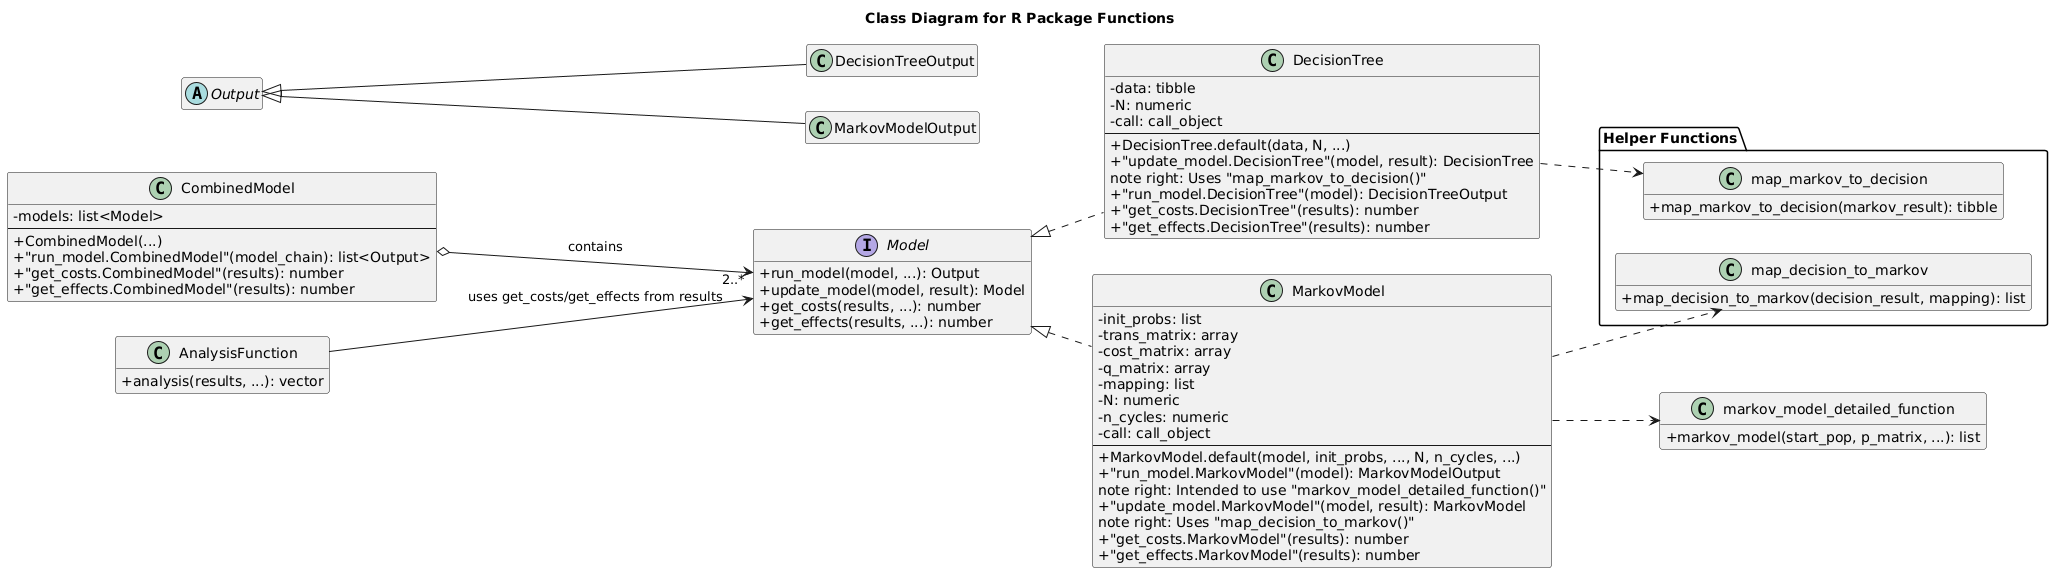
\includegraphics[width=1\textwidth,height=\textheight]{UML.png}

}

\caption{\label{fig-UML}UML diagram for the decision tree - Markov model
code. Inheritance / Generalization is a solid line with a large hollow
(unfilled) triangle arrowhead pointing to the parent class in our case
the decision tree and Markov model output; Implementation is a dashed
line with a large hollow (unfilled) triangle arrowhead pointing to the
interface, in our case the specific type of models; Dependency is a
dashed line with an open arrowhead, the function on the right hand side
of the diagram. The line with the unfilled diamond represents
aggregation and ``2..*'' indicates that there are 2 or more models in
\texttt{CombinedModel}.}

\end{figure}%




\end{document}
